% !TEX root = QlockToo.tex

\section{Konstruktion und Produktion}
\label{sec:KonstruktionFertigung}

\begin{multicols}{2}
Um die Herstellungskosten möglichst gering zu halten wird die QlockToo als eine Kombination aus Kaufteilen und eigener Produktion ausgeführt. Ziel ist eine möglichst getreue Nachbildung der Original QLOCKTWO® der Biegert~\&~Funk Manufacture GmbH \& Co. KG.

\textbf{Das Uhrgehäuse} Die Basis für das Uhrengehäuse bildet der IKEA-Bilderrahmen RIBBA in schwarz. Die Bilddarstellungsmaße von 50 x 50 cm eigenen sich gut, um die Buchstabenmatrix zur Geltung zu bringen.

{
\centering
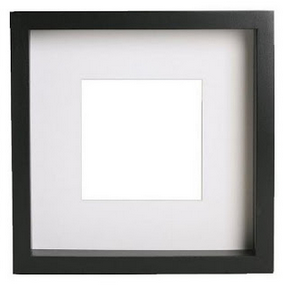
\includegraphics[width=0.75\columnwidth]{Abbildungen/Konstruktion/Ribba02} %Bilderrahmen

}
In dem besonders tiefen Rahmen,  Tiefe~=~4,5~cm, kann die komplette LED-Matrix inklusive der Elektronik untergebracht werden. Es sind lediglich keine Modifikationen notwendig.
Zum Hinausführen des Stromkabels und zur Anbringung der Taster muss der Rahmen an den entsprechenden Stellen aufgebohrt werden.

{
\centering
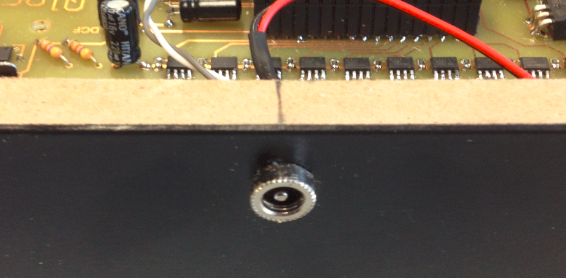
\includegraphics[width=0.6\columnwidth]{Abbildungen/Konstruktion/Stecker01}

}

{
\centering
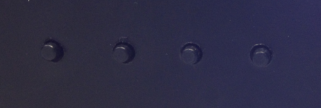
\includegraphics[width=0.6\columnwidth]{Abbildungen/Konstruktion/Taster03}

}



\textbf{Buchstabenfolie} Zur Darstellung der Zeit in Worten wird eine schwarze Folie mit einer negativen Buchstabenmatrix auf eine Plexiglasscheibe geklebt. Die Anordnung der Buchstaben entspricht der Original QLOCKTWO®.

{
\centering
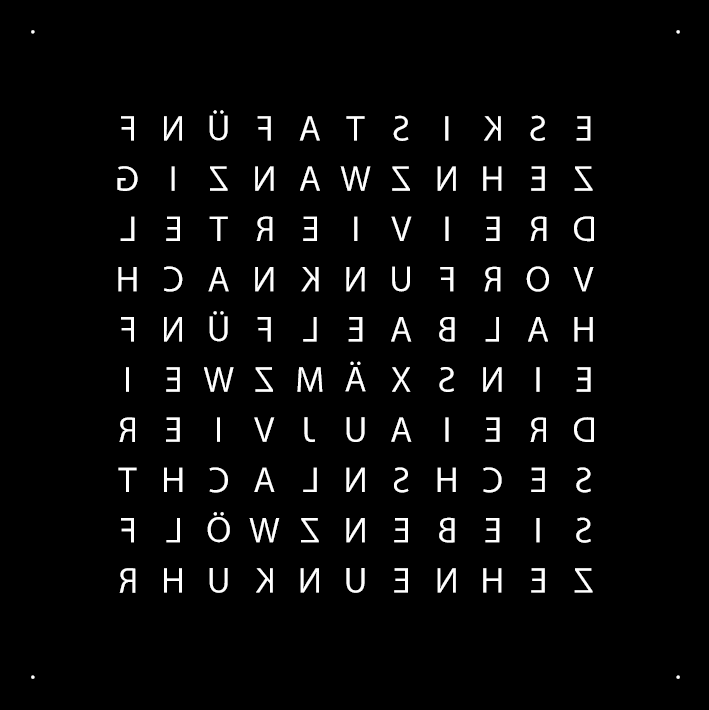
\includegraphics[width=0.75\columnwidth]{Abbildungen/Konstruktion/Buchstaben}

}
Mit der gewählten Buchstabenmatrix ist die Uhr auf eine deutsche Anzeige festgelegt. Die Original QLOCKTWO® CLASSIC beherrscht zwölf Sprachen. Durch Austauschen des Frontcovers kann die gewünschte Sprache eingestellt werden.

\textbf{LED-Matrix} Die LED-Matrix wird aus einer quadratischen MDF-Platte gefertigt. Abbildung ~\ref{fig:Spanplatte} zeigt die Fertigungs- bzw. Bearbeitungszeichnung der Spanplatte. Diese wird entsprechend der vorgegebenen Buchstabenmatrix -  10~x~11 Buchstaben - gebohrt und gesenkt, sodass die LEDs die kompletten Buchstaben ausleuchten können.

{
\centering
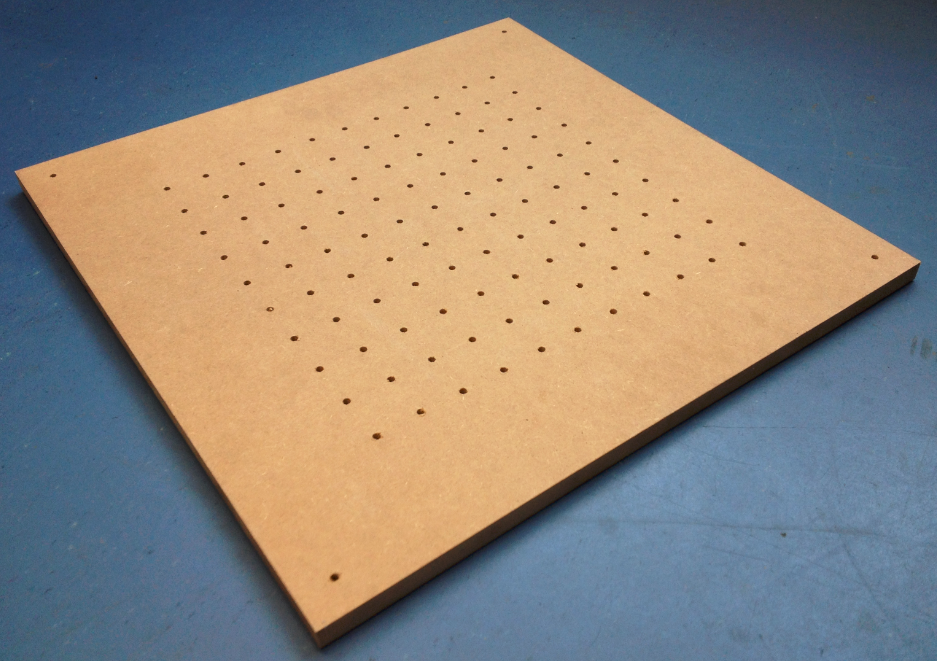
\includegraphics[width=0.8\columnwidth]{Abbildungen/Konstruktion/Platte02}

}
Für den Lichtsensor und für die Minuten-LEDs werden weitere Löcher am oberen Rand und in den vier Ecken gebohrt. Zusätzlich wird ein Ausschnitt zur Aufnahme der Platine aus der Platte gefräst.

{
\centering
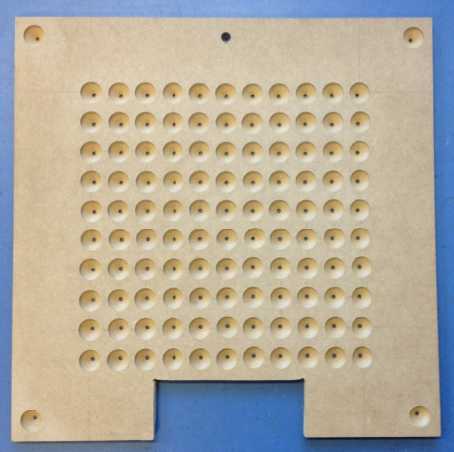
\includegraphics[width=0.85\columnwidth]{Abbildungen/Konstruktion/Platte03}

}
Die LEDs werden entsprechend hinter den Löchern positioniert, verdrahtet und mit Heißkleber fixiert. Bei der Erstellung des LED-Gitters ist darauf zu achten, dass die LED-Beinchen, Anode und Kathode, immer in die selbe Richtung zeigen.

{
\centering
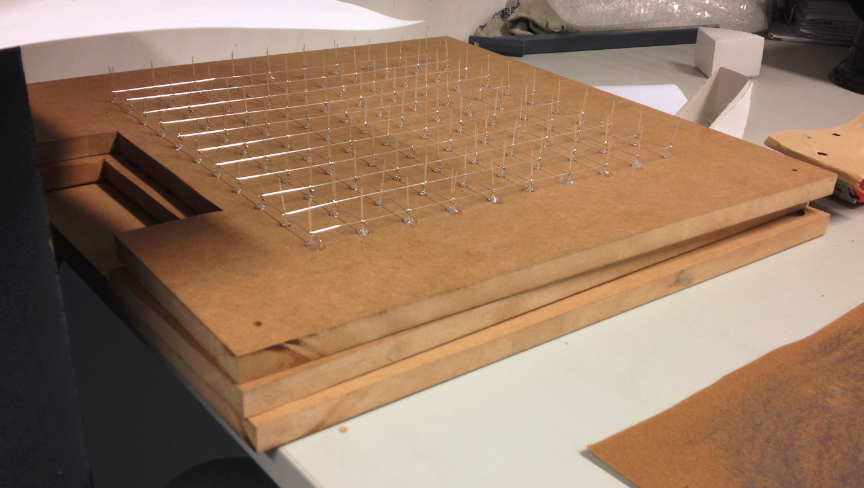
\includegraphics[width=0.85\columnwidth]{Abbildungen/Konstruktion/LED01}

}
Die Verkabelung erfolgt möglichst direkt, einfach und übersichtlich mit Flachbandkabeln.

{
\centering
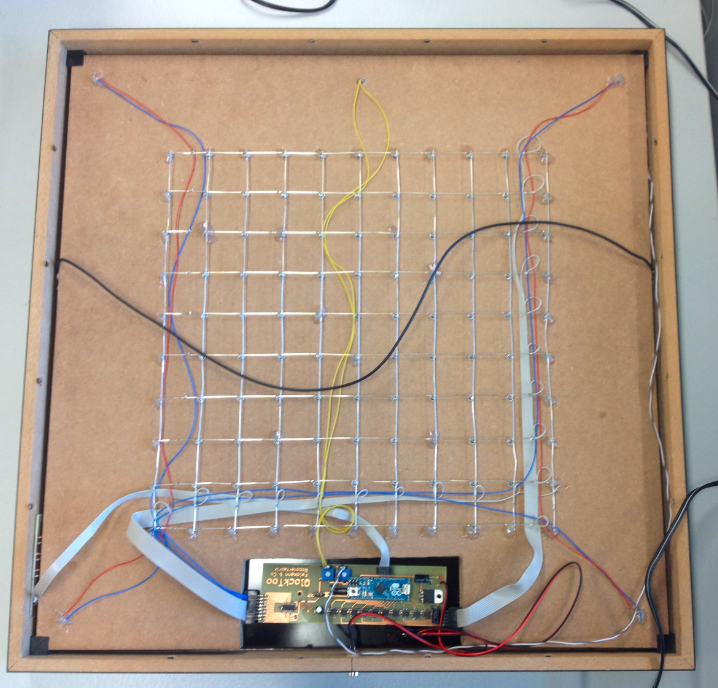
\includegraphics[width=0.85\columnwidth]{Abbildungen/Konstruktion/Platte04}

}

\textbf{LEDs} Ohne eine zusätzliche Streuung kann man die LEDs hinter den jeweiligen Buchstaben deutlich erkennen. Eine vollständige Ausleuchtung ist nicht möglich.

{
\centering
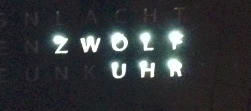
\includegraphics[width=0.85\columnwidth]{Abbildungen/Konstruktion/LED03}

}
Um eine möglichst breite Streuung des LED-Lichtes zu erzielen, wird hinter die Buchstabenfolie eine zweite Diffusorfolie  geklebt. Trotz der doppelten Folie ist die Streuung des Lichtes jedoch nicht ausreichend.

{
\centering
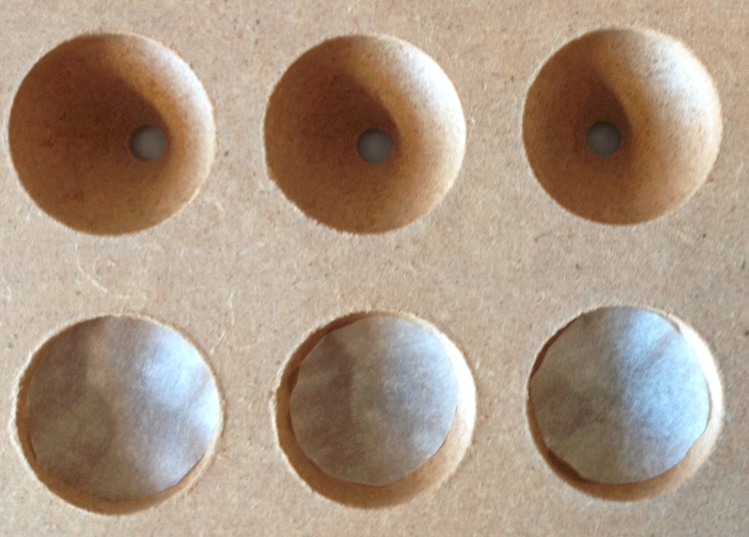
\includegraphics[width=0.6\columnwidth]{Abbildungen/Konstruktion/Diffusor01}

}
Um diese zusätzlich zu erhöhen, wird ein Streuplättchen (D:~25~mm) aus transparentem Papier in die gesenkten Kegel geklebt.

{
\centering
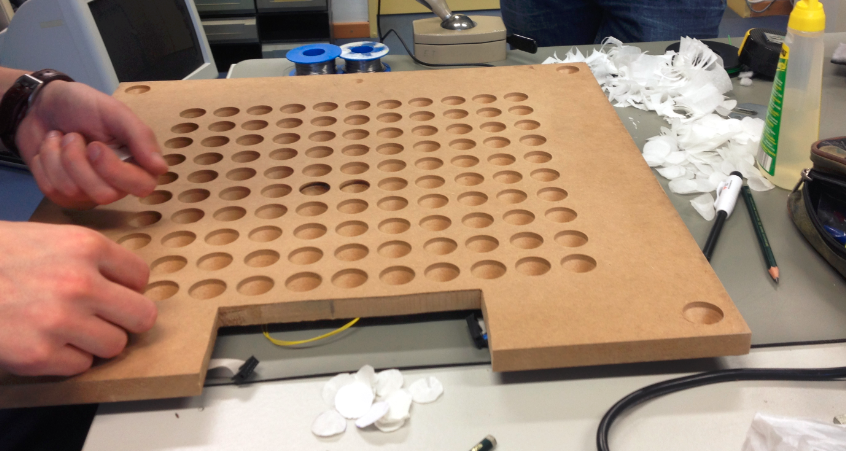
\includegraphics[width=0.85\columnwidth]{Abbildungen/Konstruktion/LED02}

}

Zur Fixierung der LED -Matrix werden Winkel aus ABS gedruckt. Diese sorgen dafür, dass die MDF-Platte in Position gehalten wird. Schlussendlich wird noch ein Kabel an die MDF-Platte geschraubt, um die Uhr an die Wand zu hängen. Diese Aufhängung ermöglicht ein gerades Ausrichten an nur einem Punkt.


\end{multicols}

\begin{landscape}
	\begin{figure}
		\centering
		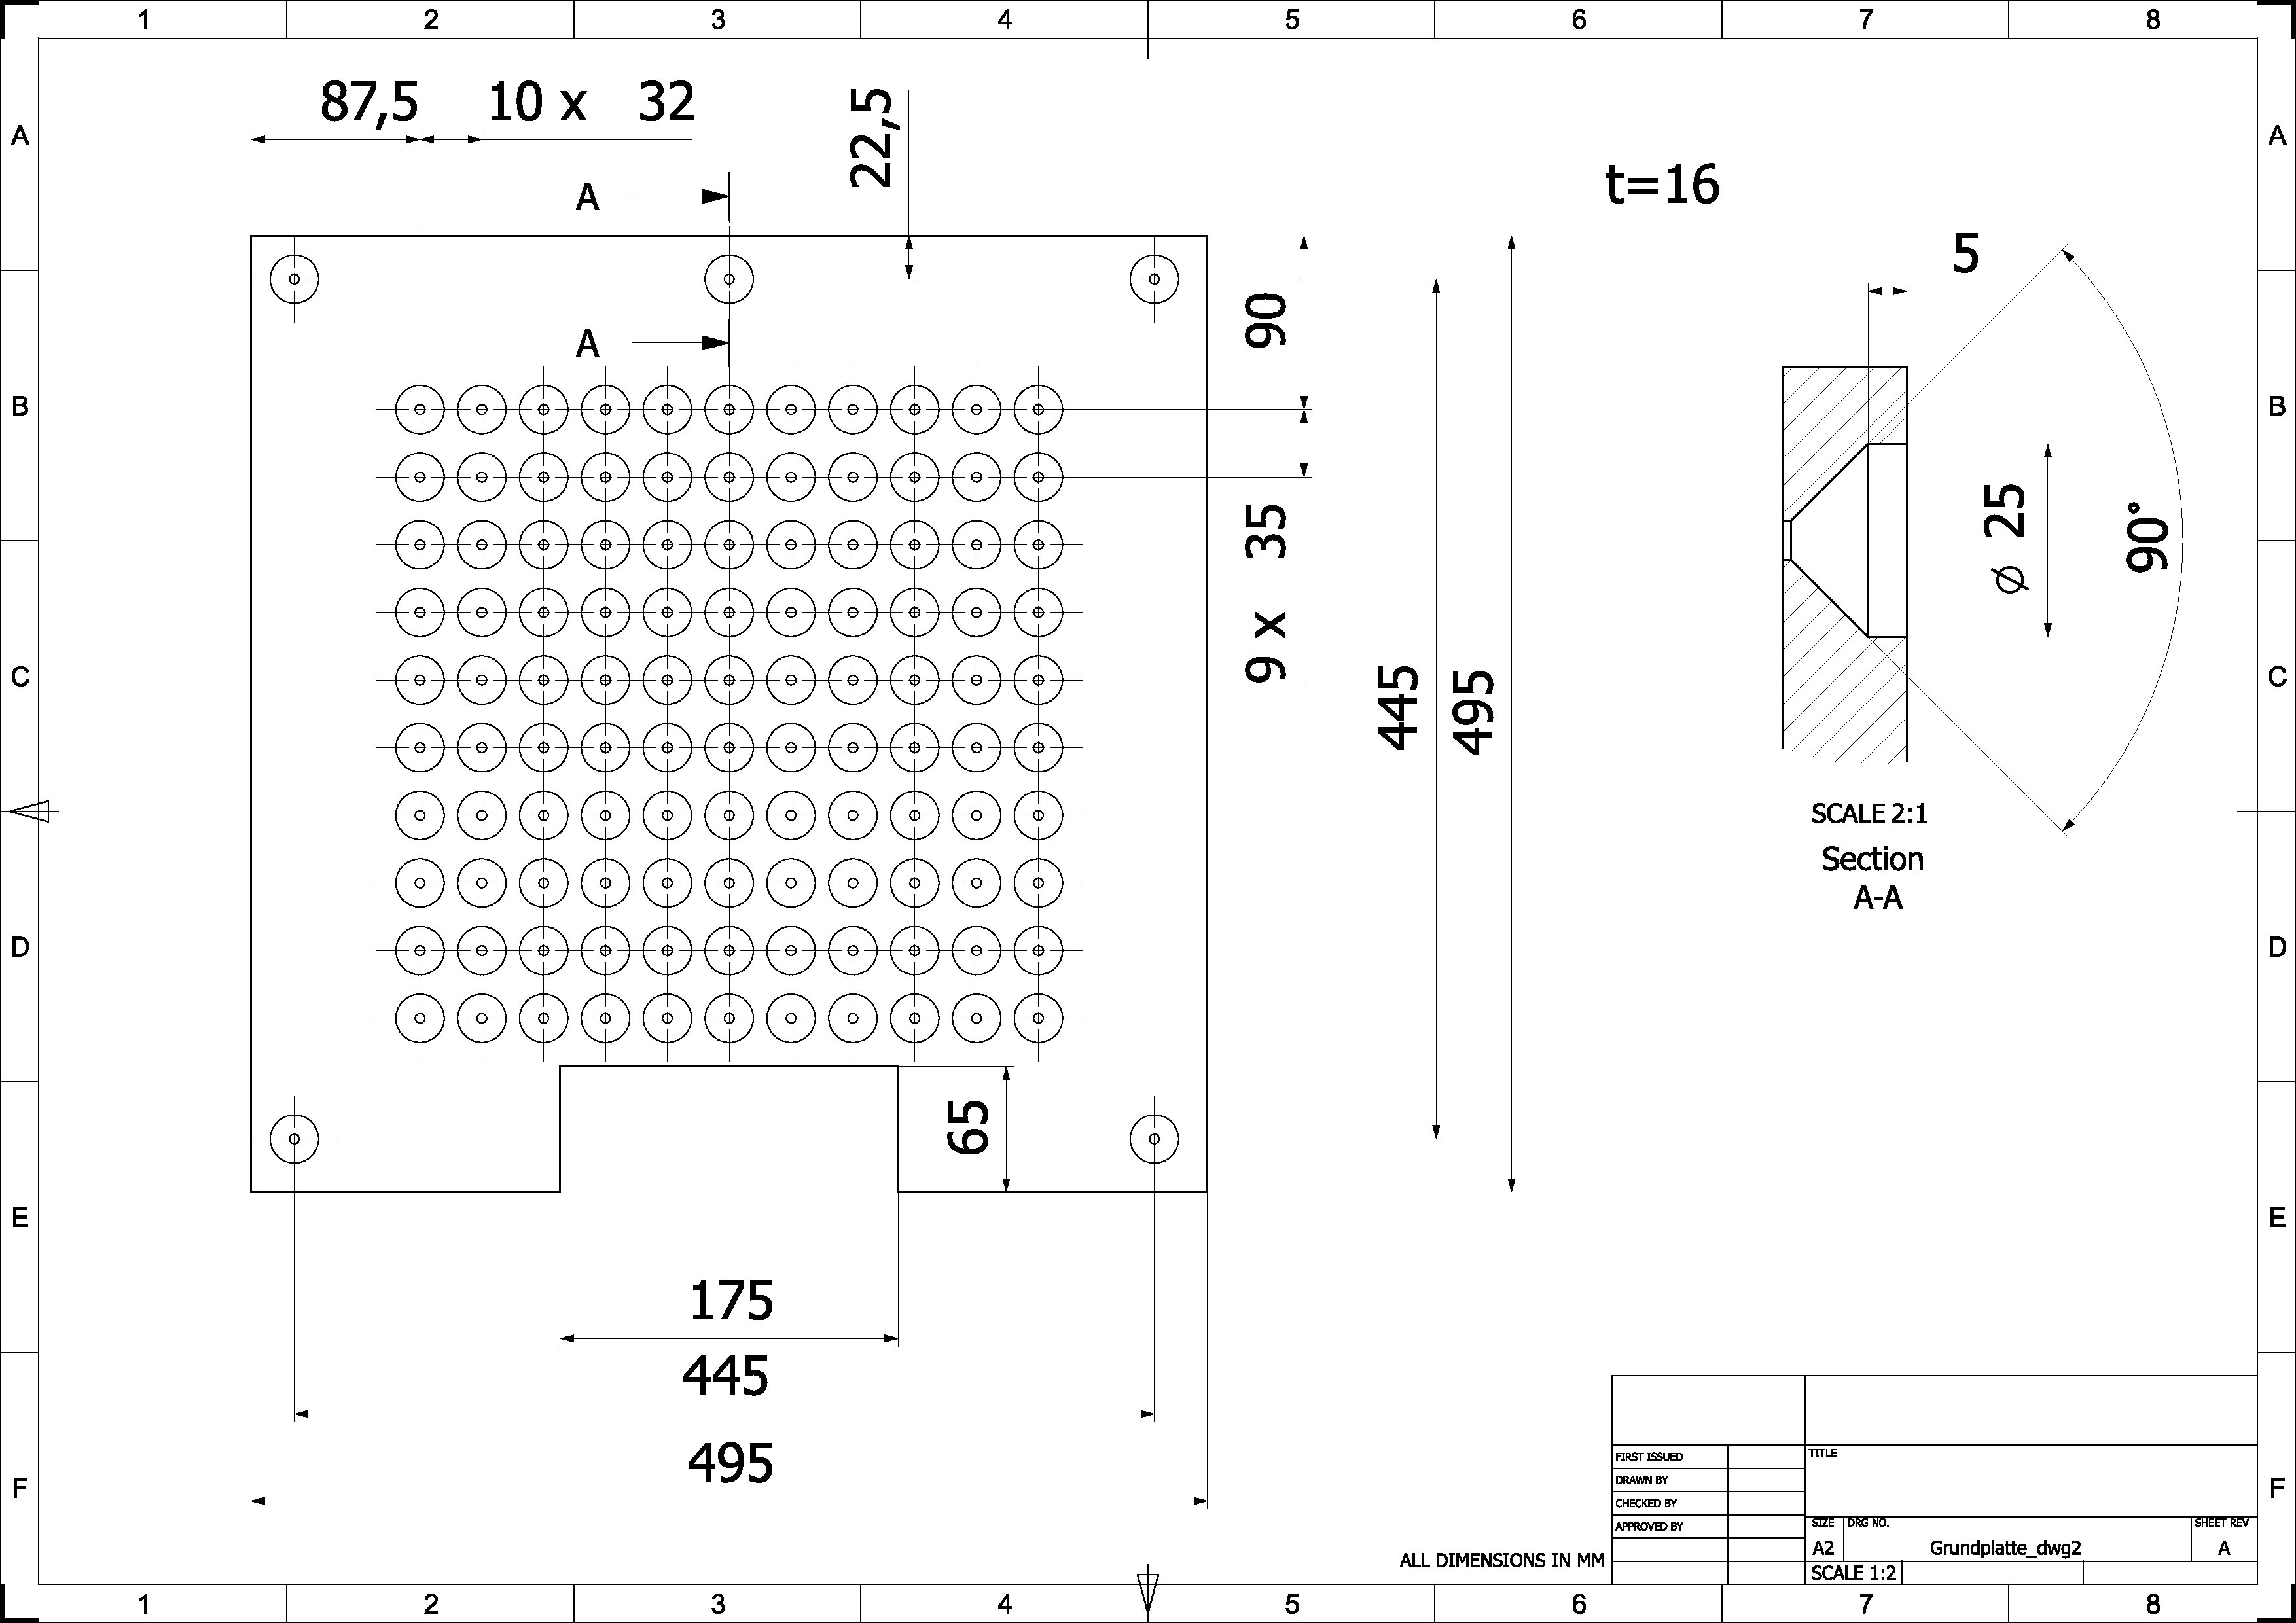
\includegraphics[width=21cm]{Abbildungen/Konstruktion/Grundplatte}
		\caption[Spanplatte]{Fertigungszeichnung Spanplatte}
		\label{fig:Spanplatte}
	\end{figure}
\end{landscape}


